\documentclass[12pt, twoside]{article}
% \documentclass[12pt, twoside]{article}
\usepackage[letterpaper, margin=1in, headsep=0.2in]{geometry}
\setlength{\headheight}{0.6in}
%\usepackage[english]{babel}
\usepackage[utf8]{inputenc}
\usepackage{microtype}
\usepackage{amsmath}
\usepackage{amssymb}
%\usepackage{amsfonts}
\usepackage[nomessages]{fp} %\FPeval{\var-name}{2*sin(pi/6)}
\usepackage{siunitx} %units in math. eg 20\milli\meter
\usepackage{yhmath} % for arcs, overparenth command
\usepackage{tikz} %graphics
\usetikzlibrary{quotes, angles, arrows, arrows.meta}
\usepackage{graphicx} %consider setting \graphicspath{{images/}}
\usepackage{parskip} %no paragraph indent
\usepackage{enumitem}
\usepackage{multicol}
\usepackage{venndiagram}

\usepackage{fancyhdr}
\pagestyle{fancy}
\fancyhf{}
\renewcommand{\headrulewidth}{0pt} % disable the underline of the header
\raggedbottom
\hfuzz=2mm %suppresses overfull box warnings

\usepackage{hyperref}

\title{PreCalculus}
\author{Chris Huson}
\date{March 2023}

\fancyhead[LE]{\thepage}
\fancyhead[RO]{\thepage \\ Name: \hspace{3cm} \,\\}
\fancyhead[LO]{BECA / Huson / Unit 11: Calculus \\* 4 April 2023}

\begin{document}

\subsubsection*{11.4 Quiz: Derivatives}
Use your own notebook, but no calculators or computers

\begin{enumerate}

\subsubsection*{Find the derivative of each polynomial function}
\item $f(x)=x^3+4x^2$ \vspace{3cm}
\item $f(x)=x^5-3x^4+2x^2$ \par \vspace{3cm}

\textbf{Evaluate the function and its derivative at a given point}
\item Given $f(x)=2x^3-5x^2$
\begin{enumerate}[itemsep=3cm]
    \item Find $f(1)$
    \item Find $f'(1)$
\end{enumerate} \vspace{2cm}

\newpage
\item The graph shows the polynomial function $\displaystyle f(x)=2x^4+5x$. Mark the portion of the function that is increasing.
    \begin{center}
    \begin{tikzpicture}[x=2cm, y=0.5cm, scale=1]
        \draw [thin, color=lightgray, xstep=1.0cm,ystep=1.0cm] (-2,-4.1) grid (2,12);
        \draw [thick, ->] (-2,0) -- (+2.1,0) node [above right]{$x$};
        \draw [thick, ->] (0,-6) -- (0,13) node [right]{$y$};
        \foreach \x in {-3,...,4}
            \draw (\x cm,0) -- (\x cm,0) node[below] {$\x$};
        \foreach \y in {-4,-2,...,12}
            \draw[shift={(0,\y)}] (2pt,0pt)--(-2pt,0pt) node[left]{$\y$};
        \draw [thick,<->,smooth,domain=-1.8:1.3] plot(\x,{(2*\x*\x*\x*\x+5*\x)});
    \end{tikzpicture}
    \end{center}

\item A function is defined over the domain $-1 \leq x \leq 4$. The function, its derivative, and graph are given as:
\begin{multicols}{2}
    $$y=-x^2+3x+2$$
    $$\frac{dy}{dx}=-2x+3$$
    \begin{enumerate}[itemsep=1cm]
        \item Find $\displaystyle \left. \frac{dy}{dx} \right|_{x=1}$
        \item Mark the portion of the function that is increasing.
    \end{enumerate}
    \begin{center}
        \begin{tikzpicture}[x=1cm, y=1cm, scale=0.9]
            \draw [thin, color=lightgray, xstep=1.0cm,ystep=1.0cm] (-2,-2) grid (4,6);
            \draw [thick, ->] (-2,0) -- (+4.1,0) node [above right]{$x$};
            \draw [thick, ->] (0,-2) -- (0,6.3) node [right]{$y$};
            \foreach \x in {-2,...,4}
                \draw (\x cm,0) -- (\x cm,0) node[below] {$\x$};
            \foreach \y in {-2,...,6}
                \draw[shift={(0,\y)}] (2pt,0pt)--(-2pt,0pt) node[left]{$\y$};
            \draw [thick,smooth,domain=-1:4] plot(\x,{(-\x*\x+3*\x+3)});
        \end{tikzpicture}
    \end{center}
    \end{multicols}

\end{enumerate}
\end{document}



